\section{The need to combine resolution and precision}
\label{sec:motivation}

Traditional data reduction techniques work by either truncating the finest few resolution levels, or
truncating the last few low-ordered bits of every sample, but rarely both. Our aim in this section
is to show that significant gain can be achieved when one combines both dimensions, namely
resolution and precision, for data reduction. To do so, for each data set, we construct and compare
three different streams, which use different sorting criteria to sort the same set of chunks in
decreasing order of weights. We will use $W(c)$ to denote a sorting criteria, which is any function
that takes a chunk, $c$, and returns its `'weight'', which determines how important the chunk is.

The weight function used by the first stream is $W_1(c)=\bar{l}-L(c)$, where $L$ is a function that
returns the subband (resolution level) of its argument (higher-numbered subbands are finer), and
$\bar{l}$ is the total number of subbands. This stream orders the chunks strictly from coarser to
finer resolution levels, so we will name it the \emph{by level} stream. Within the same subband,
without any further knowledge of the underlying data, the chunks naturally follow the row-major
order. The second stream, \emph{by bit plane}, proceeds stricly from higher-ordered to lower-ordered
bit planes (i.e., $W_2(c)=\bar{b}-B(c)$, where $B$ is a function that map its argument to the
corresponding bit plane and $\bar{b}$ is the total number of bit planes, with $0$ being the most
significant bit plane). The third stream, \emph{by wavelet norm}, orders chunks using
$W_3(c)=2^{\bar{b}-1-B(c)}\times \norm{\omega_{L(c)}}^2$. The term $2^{\bar{b}-1-B(c)}$ captures the
contribution of a bit on bit plane $B(c)$, while the term $\norm{\omega_{L(c)}}^2$ captures the
contribution of a coefficient on subband $L(c)$, where $\omega_{L(c)}$ refers to the wavelet basis
function on subband $L(c)$. Note that all three streams are data-agnostic, and the \emph{by level}
and \emph{by bit plane} streams are designed to mimic the way data is read in traditional data
reduction methods that work either in resolution or in precision space, while \emph{by wavelet norm}
combines these two dimensions. Finally, to emulate the effect of entropy compression typically done
in practice, we remove all the chunks that consist of purely leading zero bits from all streams.

We compare the three streams by plotting an error curve for each, with regards to three error
metrics, namely root-mean-square error (Figure \ref{fig:motivation-rmse}), histogram error (Figure
\ref{fig:motivation-histogram}), and isocontour error (Figure \ref{fig:motivation-isocontour}). For
each metric, the function is reconstructed every time a new chunk is received from a stream, then
the relevant quantity (the function itself, its histogram, or an isocontour) is computed from the
reconstructed function, and compared against the same quantity computed from the original (lossless)
function. The definitions of histogram error and isocontour error are discussed in detail in Section
[REF] and Section [REF] respectively.

\begin{figure}
  \centering
	\subcaptionbox{Boiler}
  {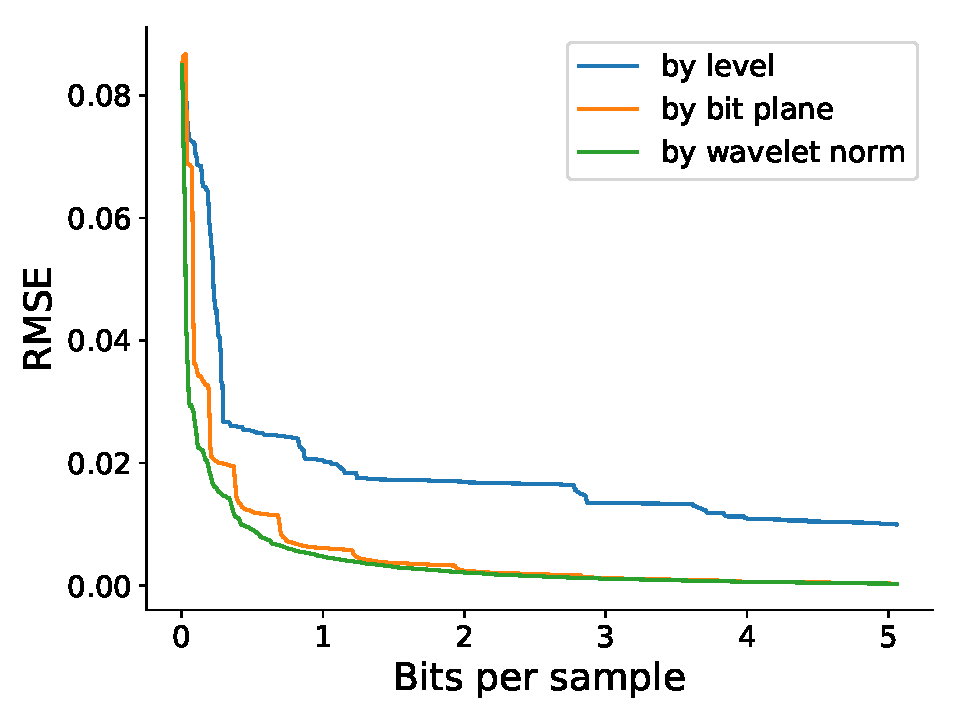
\includegraphics[width=0.48\linewidth]{img/motivation/motivation-psnr-boiler.pdf}}
	\subcaptionbox{Diffusivity}
 	{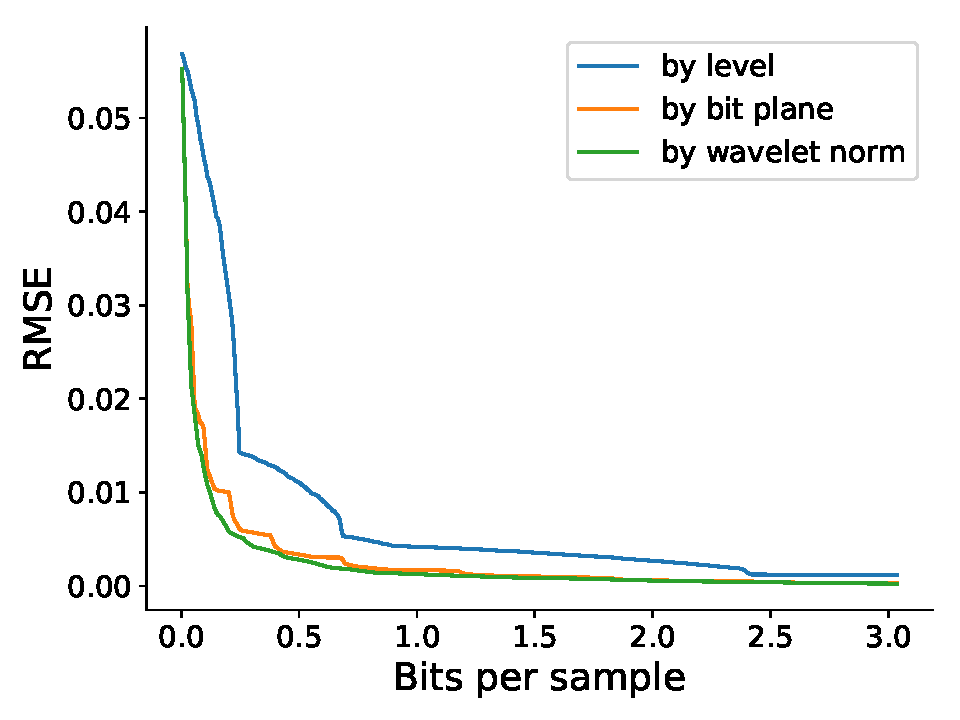
\includegraphics[width=0.48\linewidth]{img/motivation/motivation-psnr-diffusivity.pdf}}
	\subcaptionbox{Euler}
 	{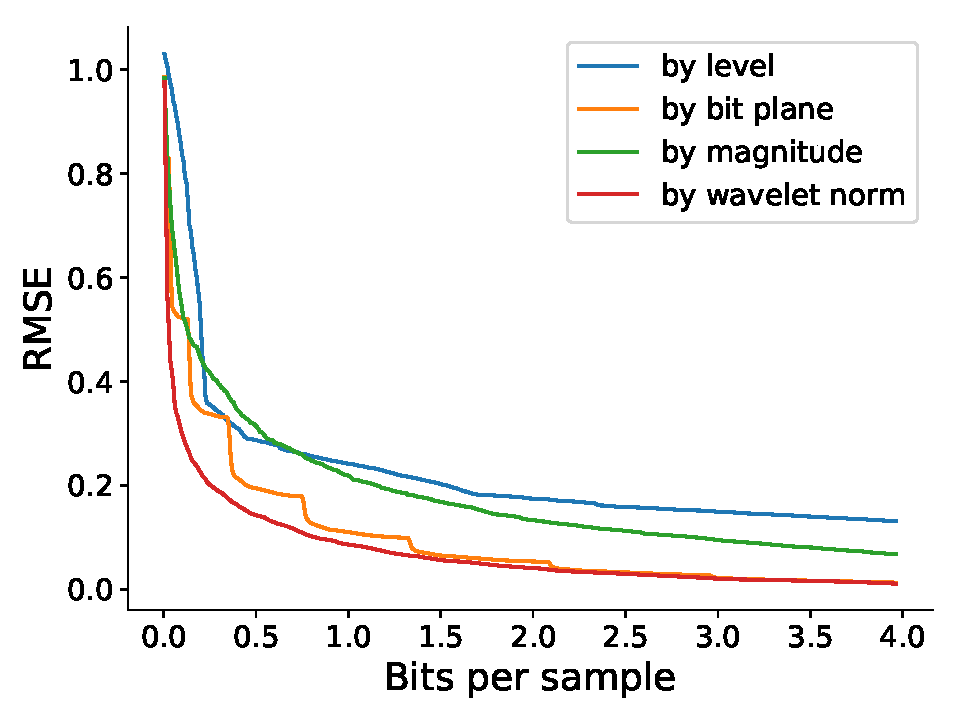
\includegraphics[width=0.48\linewidth]{img/motivation/motivation-psnr-plasma.pdf}}
	\subcaptionbox{Turbulence}
 	{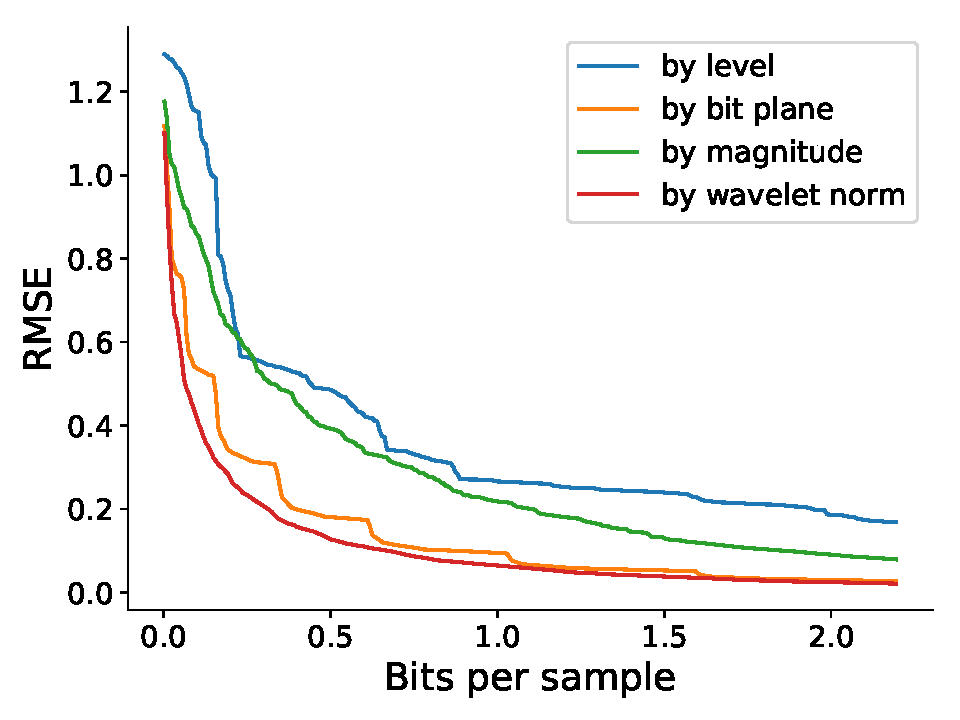
\includegraphics[width=0.48\linewidth]{img/motivation/motivation-psnr-turbulence.pdf}}
	\subcaptionbox{Plasma}
 	{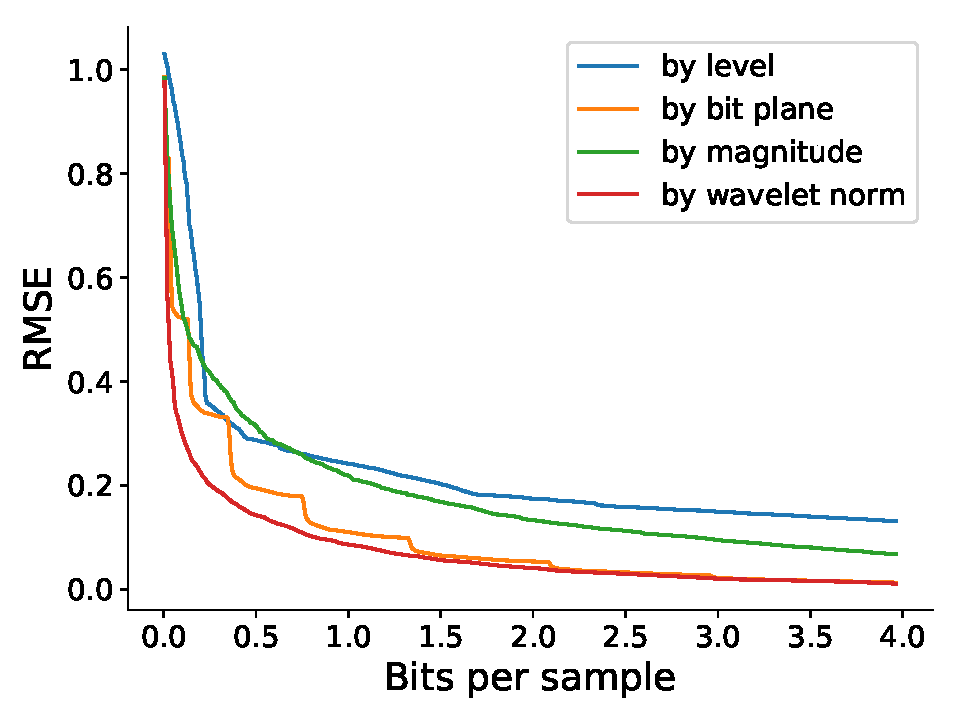
\includegraphics[width=0.48\linewidth]{img/motivation/motivation-psnr-plasma.pdf}}
	\subcaptionbox{Velocity-z}
 	{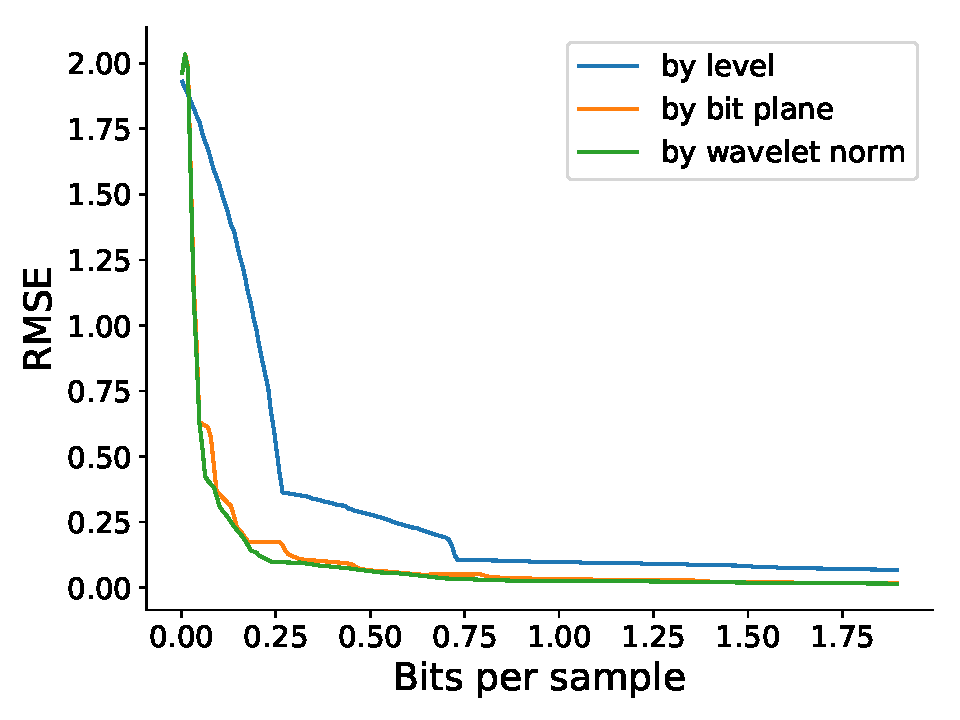
\includegraphics[width=0.48\linewidth]{img/motivation/motivation-psnr-velocityz.pdf}}
 	\caption{Root-mean-square error of reconstructed functions using the three data-agnostic streams
 	defined in Section \ref{sec:motivation}. Lower is better. The streams are truncated to highlight
 	the differences, without omitting important information. \emph{by wavelet norm} performs best,
 	followed closely by \emph{by bit plane}.}
 	\label{fig:motivation-rmse}
\end{figure}

\begin{figure}
  \centering
	\subcaptionbox{Boiler}
  {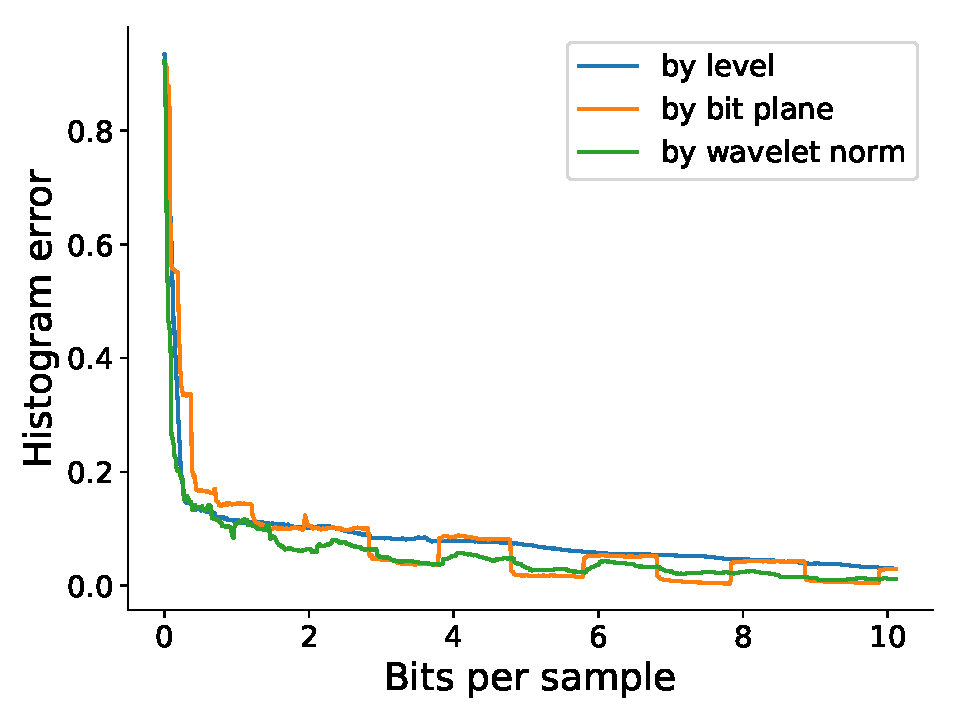
\includegraphics[width=0.48\linewidth]{img/motivation/motivation-histogram-boiler.pdf}}
	\subcaptionbox{Diffusivity}
 	{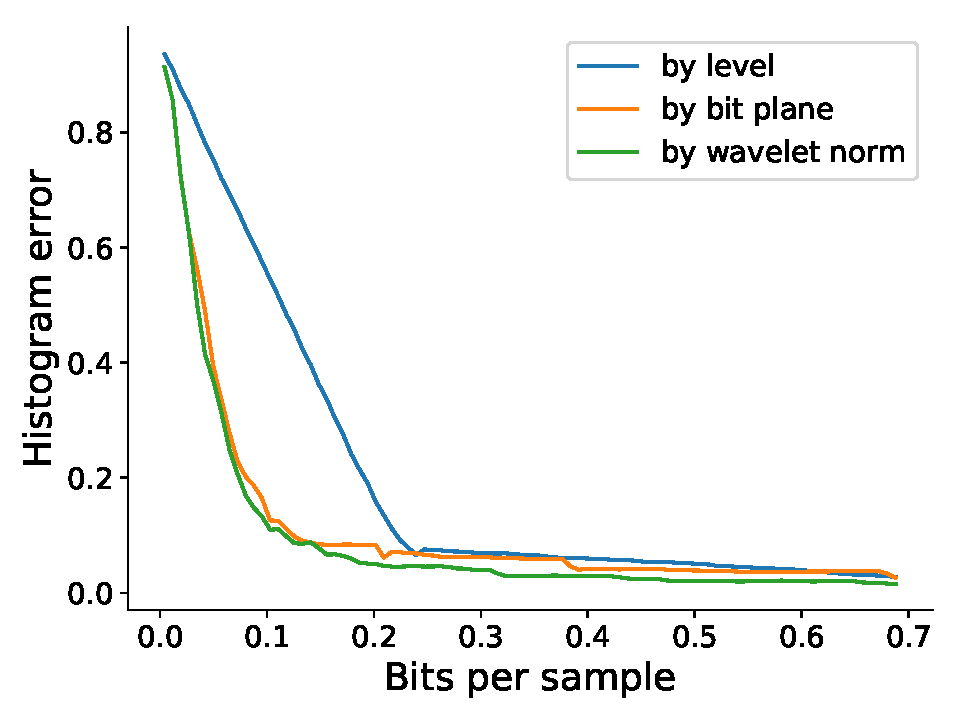
\includegraphics[width=0.48\linewidth]{img/motivation/motivation-histogram-diffusivity.pdf}}
	\subcaptionbox{Euler}
 	{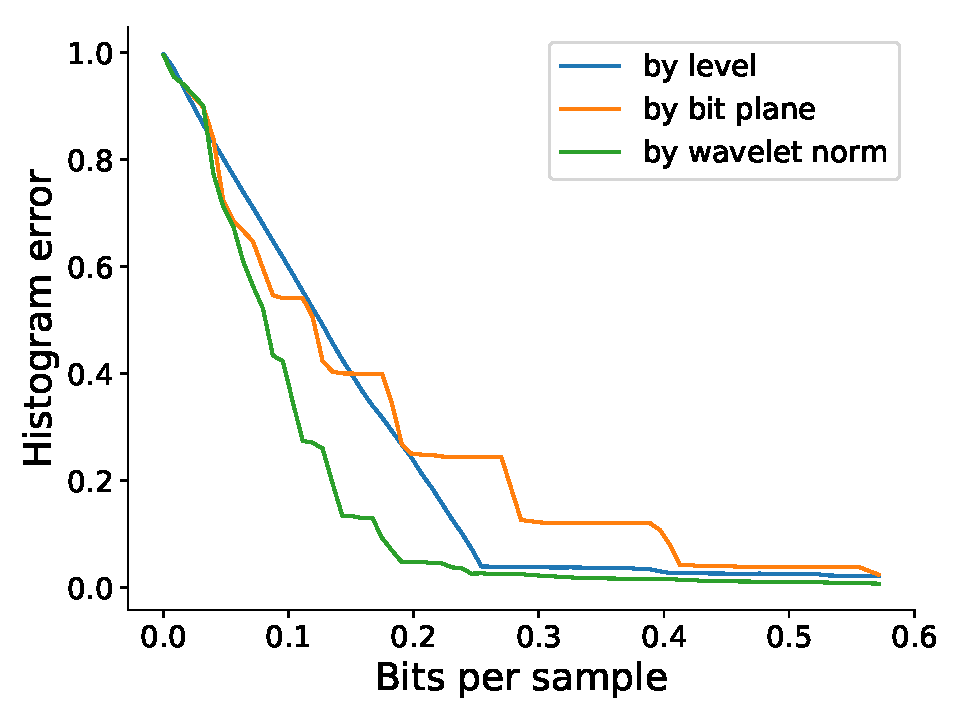
\includegraphics[width=0.48\linewidth]{img/motivation/motivation-histogram-euler.pdf}}
	\subcaptionbox{Turbulence}
 	{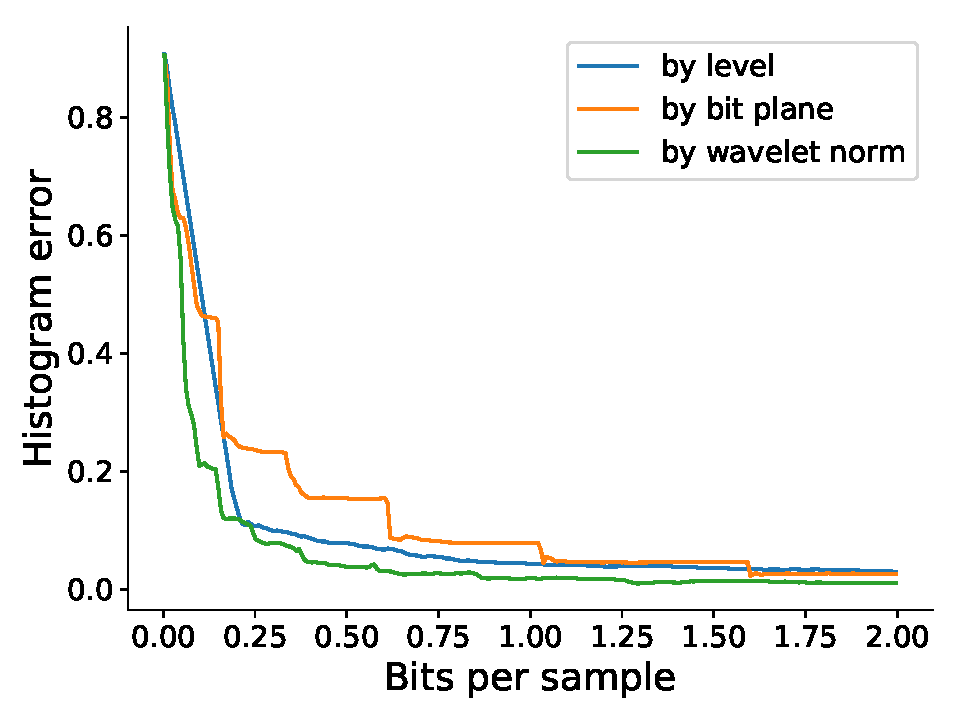
\includegraphics[width=0.48\linewidth]{img/motivation/motivation-histogram-turbulence.pdf}}
	\subcaptionbox{Plasma}
 	{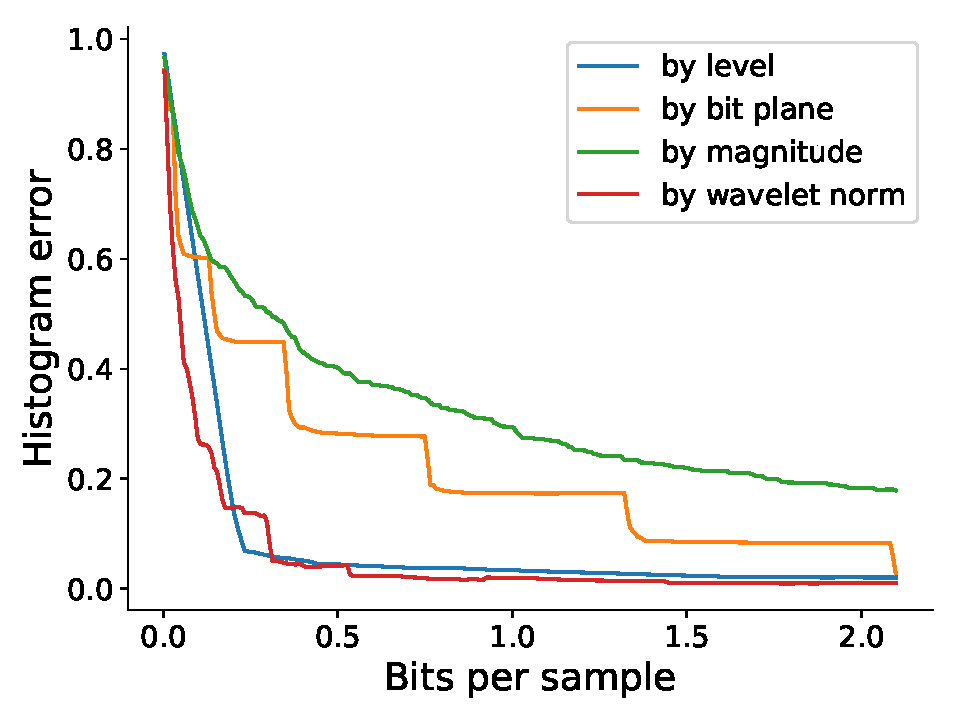
\includegraphics[width=0.48\linewidth]{img/motivation/motivation-histogram-plasma.pdf}}
	\subcaptionbox{Velocity-z}
 	{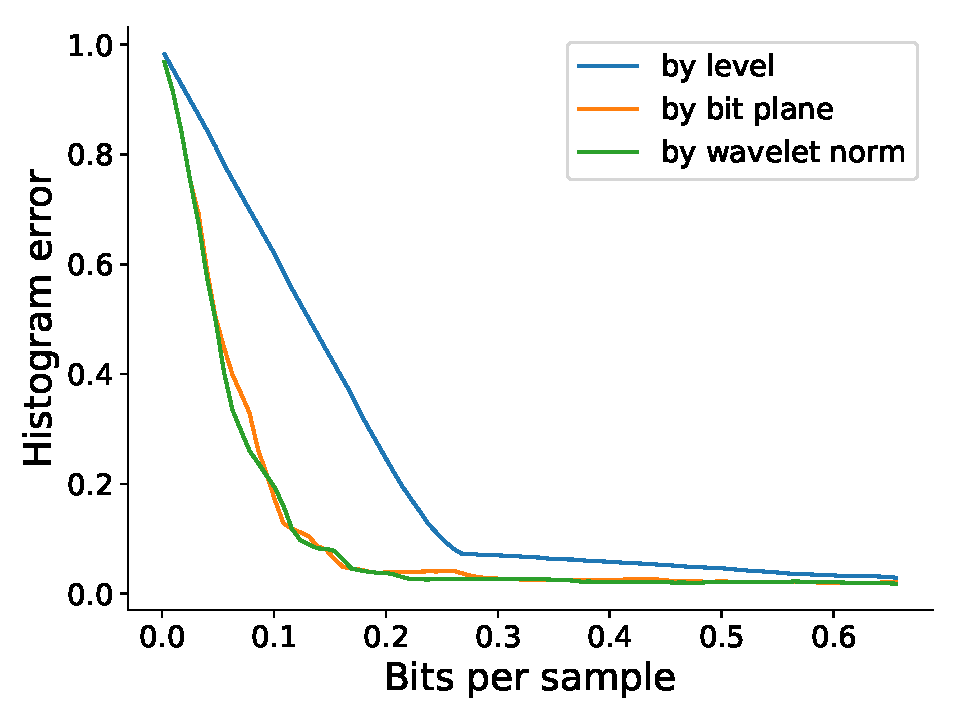
\includegraphics[width=0.48\linewidth]{img/motivation/motivation-histogram-velocityz.pdf}}
 	\caption{Histogram error of reconstructed functions using the three data-agnostic streams defined
 	in Section \ref{sec:motivation}. Lower is better. Each histogram comprises of 256 bins. The
 	streams are truncated to highlight the differences, without omitting important information.
 	\emph{by wavelet norm} performs best.}
 	\label{fig:motivation-histogram}
\end{figure}

\begin{figure}
  \centering
	\subcaptionbox{Boiler, isovalue = $0.07$}
  {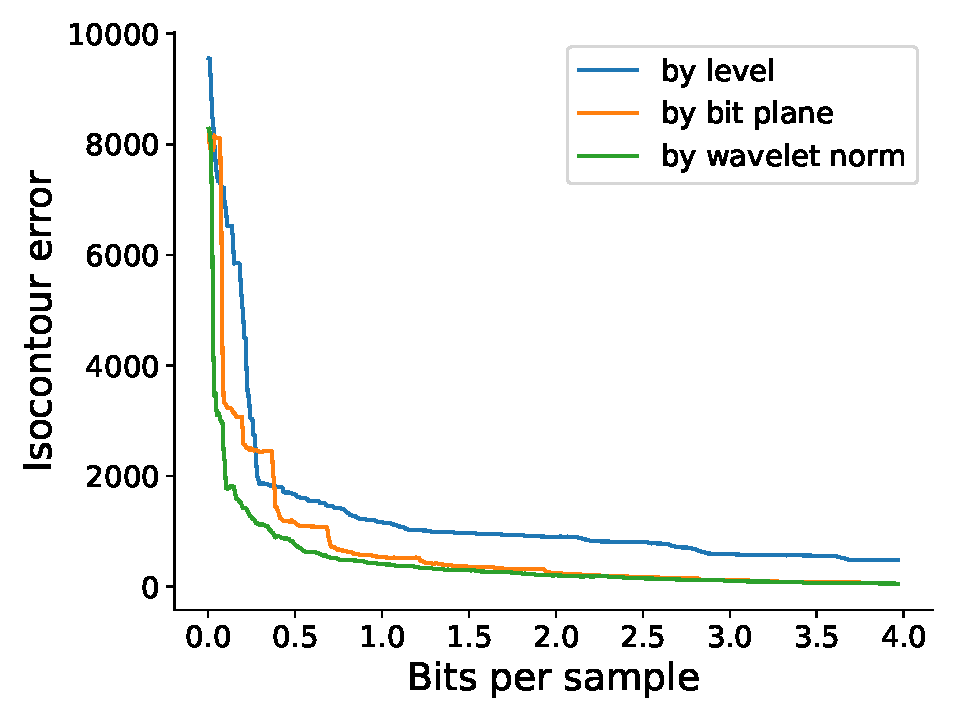
\includegraphics[width=0.48\linewidth]{img/motivation/motivation-isocontour-boiler.pdf}}
	\subcaptionbox{Diffusivity, isovalue = $0.04315$}
 	{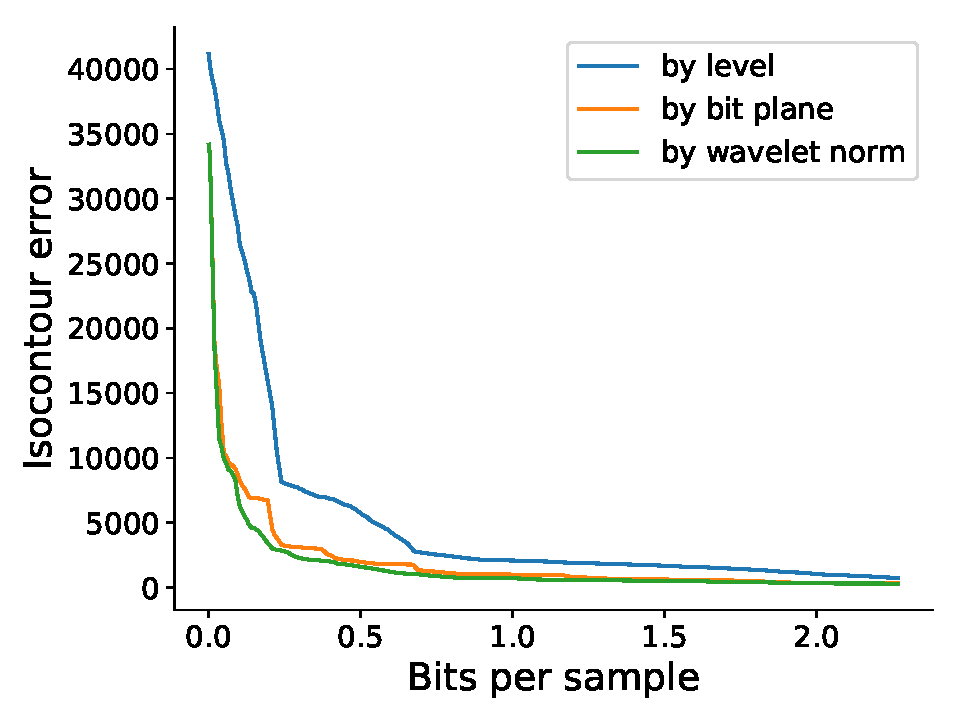
\includegraphics[width=0.48\linewidth]{img/motivation/motivation-isocontour-diffusivity.pdf}}
	\subcaptionbox{Euler, isovalue = $3$}
 	{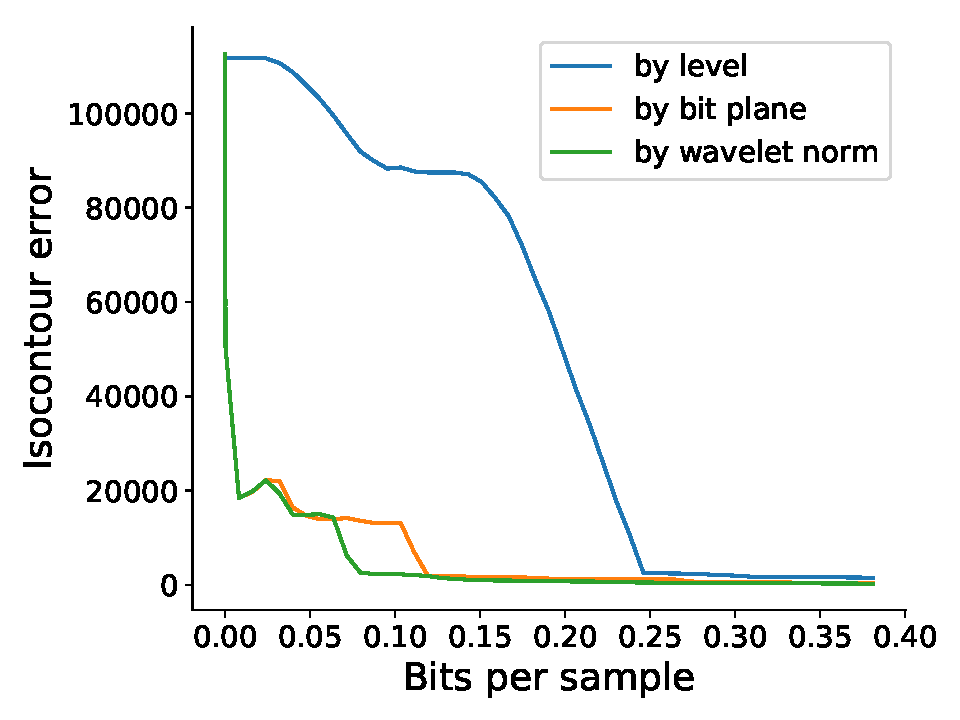
\includegraphics[width=0.48\linewidth]{img/motivation/motivation-isocontour-euler.pdf}}
	\subcaptionbox{Turbulence, isovalue = $2$}
 	{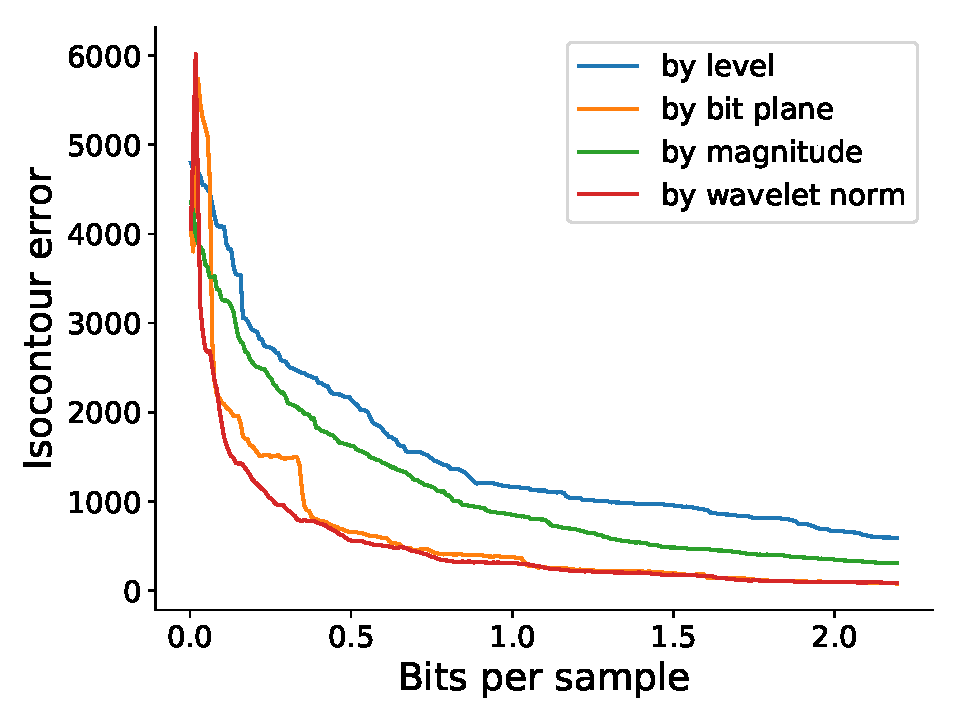
\includegraphics[width=0.48\linewidth]{img/motivation/motivation-isocontour-turbulence.pdf}}
	\subcaptionbox{Plasma, isovalue = $2$}
 	{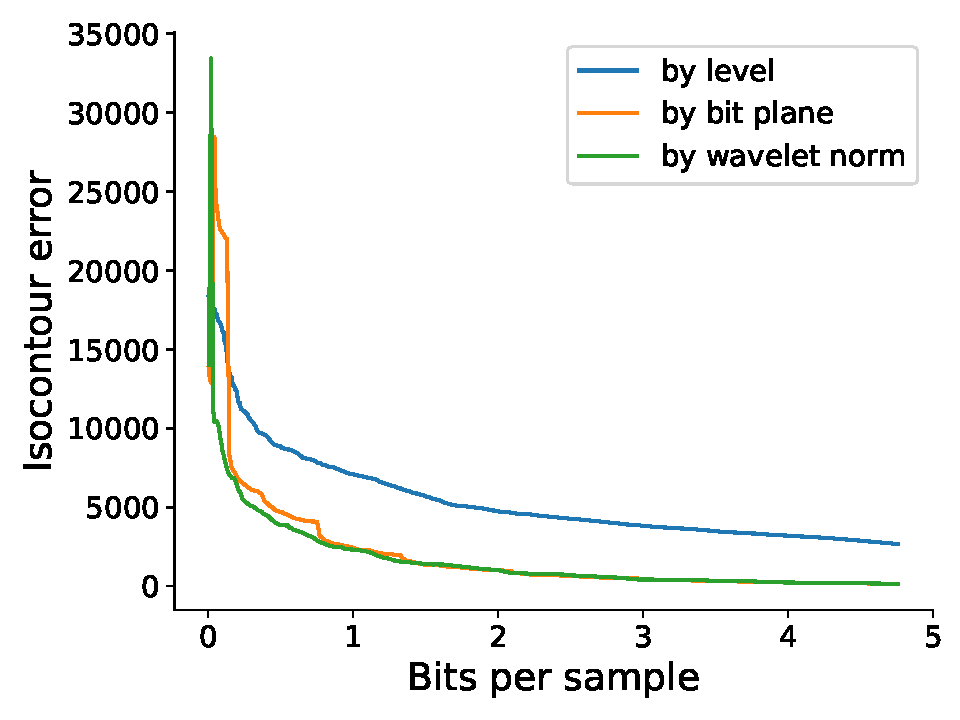
\includegraphics[width=0.48\linewidth]{img/motivation/motivation-isocontour-plasma.pdf}}
	\subcaptionbox{Velocity-z, isovalue = $-2$}
 	{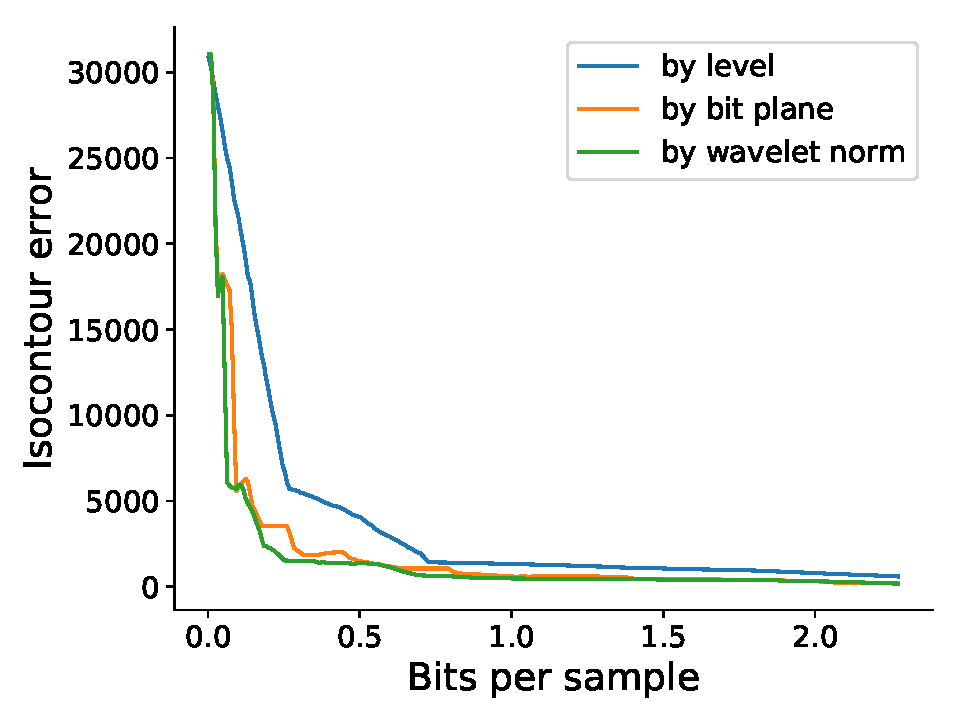
\includegraphics[width=0.48\linewidth]{img/motivation/motivation-isocontour-velocityz.pdf}}
 	\caption{Isocontour error of reconstructed functions using the three data-agnostic streams defined
 	in Section \ref{sec:motivation}. Lower is better. The streams are truncated to highlight the
 	differences, without omitting important information. \emph{by wavelet norm} performs best.}
 	\label{fig:motivation-isocontour}
\end{figure}

It can be seen that, for all metrics, the \emph{by wavelet norm} stream consistently performs the
best. The \emph{by bit plane} works almost as well as \emph{by wavelet norm} for RMS error and
isocontour error, but not for histogram error. \emph{by level} works poorly in almost all cases.
These results show that it is often suboptimal to stream or reduce data exclusively in either
resolution or precision. Combining these two dimensions of data reduction can lead to significant
quality improvement at the same bit rate, especially when quantities of interest other than simply
the function itself are considered. The reason is that \emph{by wavelet norm} can take advantage of
the fact that a higher-ordered bit from a fine-scale coefficient could contribute more than a
lower-ordered bit from a coarse-scale coefficient (which \emph{by level} ignores), and vice-versa
(which \emph{by bit plane} ignores). It is unclear, however, whether \emph{by wavelet norm} is the
best stream to use in all cases. To answer this question, we will expand our study from
data-agnostic to data-dependent streams that are optimized for each of these quantities of interest.
While data-dependent streams are likely unrealizable in practice due to the fact that the
`'receiver'' of data does not have access to the data beforehand, we hope they provide insights for
designing streams that improve on the generic \emph{by wavelet norm}, by being tailored to each
error metric.
